%% aps to author template--please use pdflatex to edit then to pdf--------------
\documentclass[fontset=ubuntu,A4,twoside]{ctexart}
%\usepackage{slashbox}\usepackage{makecell}\usepackage{diagbox}\backslashbox
\usepackage{aappss}\usepackage{epstopdf}
%\renewcommand\baselinestretch{1.235}\protect
\renewcommand\baselinestretch{2.0}\protect
\abovedisplayshortskip 0 pt plus 3pt
\belowdisplayshortskip 6 pt plus 2pt minus 2pt
\abovedisplayskip 6 pt plus 2pt minus 2pt
\belowdisplayskip 6 pt plus 2pt minus 2pt
% \info{2015}{64}{1}{01{}} \infodate{2015.0.0.}{2015.0.0.}
%=================== Text begin here ==============================
\begin{document}\apsname

\title{自动微分 \fivestar}%{\cfundlink}

\author{关云长$^{1)2)}$ \quad 刘备$^{1)\dag}$ \quad 诸葛亮$^{2)}$}

\address{1)}{山西大学光电研究所, 量子光学与光量子器件国家重点实验室, 太原 \quad 030006}

\address{2)}{清华大学物理系, 北京 \quad 100084}

%\address{3)}{}

\abstract{中文摘要. 300---400字,摘要中不用缩略词, 不用第一人称. 中英文摘要的结构建议包括: (1) 研究背景和目的; (2)方法; (3) 主要结果; (4) 结论. 简明扼要不分段, 突出结论、成果.}

\keywords{关键词1, 关键词2, 关键词3, 关键词4 (不超过4个, 与英文Keywords一一对应)}

\pacs{02.10.Yn, 33.15.Vb, 98.52.Cf, 78.47.dc \quad (不超过4个,首码须与本文所研究的专业领域一致, PACS代码可在期刊网站下载中心下载)}

\cfund{国家重点基础研究发展计划(批准号: 2011CB00000)、国家自然科学基金(批准号:
123456, 567890)和国家高技术研究发展计划(批准号: 2011AA06Z000)资助的课题.
(基金名称规范请在本刊网站下载参考``相关基金规范全称'').}

\cmail{aaa@bbb.ccc \quad }

%\cmailddag{mail2}

%\mail{}{}\cmail \cmailddag

%\apscopyright \baselineskip=16.0pt plus.2pt minus.2pt
%\begin{multicols}{2}\sec
\section{引~~~~言}


20世纪80年代以来, 量子光学发展了若干种方法: 冷原子云释放再俘获(release and
recapture, 简记为RR)$^{[1]}$、冷原子云受迫振荡$^{[2]}$、 冷原子光谱分析$^{[3]}$、非平衡四波混频$^{[4]}$、飞行时间光谱(time
of flight, TOF)$^{[5]}$ 和二维飞行时间吸收成像$^{[6]}$等. 引言的写作直接影响到读者对文章进一步了解的兴趣, 建议包括以下内容:
(1)本研究领域背景的综述; (2)其他学者已有研究成果的详细描述;
(3)陈述为什么需要进行更多的或进一步的研究;
(4)阐述作者本项研究的目的和创新性; (5)简述本文开展的研究工作;
(6)本项研究结果的意义(可选项). 特别指出的是, 希望在引言部分介绍和引用国内外物理类期刊中本研究领域的最新研究成果, 以帮助读者清楚了解该领域的最新进展及本文的创新点.

\section{中性原子模型}

\subsection{理论模型}

中性原子磁光在六维相空间中冷原子云的初始概率分布可近似表示为$^{[7]}$
\begin{eqnarray}
N(x_0, y_0, z_0; v_{x0},v_{y0}, v_{z0}) & = & \prod\limits_{i \in \{x\}}
g(i_0,  \sigma _{i0}) \cdot g(v_{i0},  \sigma _{iv}), \\
N(x_{1}, y_{1}, z_{1}; v_{x{1}}, v_{y{1}}, v_{z_{1}}) & = & \prod\limits_{i \in \{y\}} g(i_0,\sigma_{i0}) \cdot g(v_{i0}, \sigma _{iv}),
\end{eqnarray}
其中, $g(i_0, \sigma _{i0})$和$g(v_{i0}, \sigma _{iv})$为Gauss分布函数.


\subsection{实~~验}

******如图1所示.



\centerline{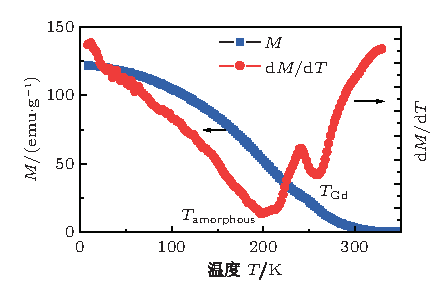
\includegraphics{fig1.eps}}
%\vspace*{6mm}

\vskip 2mm

\centerline{\footnotesize 图1\ \ \  Gd$_{60}$Fe$_{30}$Al$_{10}$条带的磁化曲线 \quad (origin等软件绘制的插图)}

\vskip 2mm

\centerline{\parbox[c]{10cm}{\footnotesize Fig.~1.~Magnetization cures of Gd$_{60}$Fe$_{30}$Al$_{10}$ band. [图题要求中英文对照,中文在前,英文在后.]
[关于图的具体要求,可详见本刊“对图的要求”.]}}

\vskip 0.55\baselineskip
%\begin{multicols}{2}


\section{实验系统及测量结果}


*****如图2所示.

分析计算得到结果如表1所示.

\newpage

%\end{multicols}
\begin{center}
\begin{footnotesize}

%\tabinfo{1}
\parbox[c]{7cm}{表1 \ \ \ 不同流体对应的等价毛细管结构参数比较}

\parbox[c]{12cm}{Table 1. Structural parameters of capillary of different kind of fluid. [表题中英文对照,中文在上,英文在下]}


\vskip 2mm \renewcommand{\arraystretch}{1.15} \tabcolsep 12pt
\centerline{
\begin{tabular*}{0.85\textwidth}{ccccccccccccc}\toprule
\raisebox{-1.50ex}[0cm][0cm]{流体类型} & \multicolumn{2}{c}{直管} &
& \multicolumn{2}{c}{分形毛细管}  \\\cline{2-3} \cline{5-6}
 & $R$/cm& $L$/cm & &  $R$/cm& $L_{0}$/cm \\ \hline
HB流体($\mu = 1.0$, $\tau _0 = 0.1$, $n = 0.8$) & 0.097 & 0.501
&& 0.124 & 1.0 \\\hline
宾汉姆流体($\mu = 1.0$, $\tau _0 = 0.1$, $n = 1$) & 0.112&
0.905 & & 0.124& 1.0 \\ \hline
幂律流体($\mu = 1.0$, $\tau _0 = 0$,$n = 0.8$) & 0.097 & 0.501&
& 0.124 & 1.0 \\\bottomrule
\multicolumn{5}{l}{注1: } % \raisebox{1.8ex}[0mm][0mm]{}
\end{tabular*}}
\end{footnotesize}
\end{center}
%\begin{multicols}{2}



%\end{multicols}
\vspace*{5mm}

\centerline{\includegraphics{fig2.eps}}
%\vspace*{6mm}

\vskip 2mm

\centerline{\parbox[c]{11cm}{\footnotesize  图2\ \ \ 电场幅值分布 \ \ \ (a) 长轴共线之$\gamma_{75}$面;(b) 短轴共线之$\gamma_{75}$面; (b) 长短轴共线之$\gamma_{75}$面;(d) 长短轴共线之$\alpha$面 \\
Fig.~2.~Distribution of the electric field intensity: (a) $\gamma_{75}$ plane of the long collinear axis; (b) $\gamma_{75}$ plane of the short collinear axis; (c)
$\gamma_{75}$ plane of the long-short collinear axis; (d) $\alpha$ plane of the
long-short collinear axis. {[分图题也要求中英文对照]}}}

\vskip 0.55\baselineskip
%\begin{multicols}{2}

\section{结~~~~论}

在研究结果与讨论的基础上总结出本研究得到的重要论点, 建议可包括以下内容:
(1)解释结果; (2)将结果与之前提出的研究目的或假设相联系,阐明结果的重要性;
(3)将结果与其他已有研究工作进行比较;
(4)尽可能得出一个很清晰的结论. 对每一个结论需要总结证据.
同时也可以指出本工作的不足和将要开展工作的展望.
请注意不能简单重复摘要和引言.

\section*{致谢}

感谢北京大学力学系某某教授和某某博士以及某某的讨论.


\section*{附录A1}

标题排列和编号方式为A1, A2, A3.

\section*{附录A2}
%
%text text
%
%\section*{附录B1}
%%\section*{附录B2}
%
%text text
%
%\section*{致谢}
%
%text text

\bigskip
%\begin{footnotesize}
\begin{thebibliography}{999}%\refmark
%\itemsep=-2pt plus.2pt minus.2pt

\bibitem{1} Chu S, Hollberg L, Bjorkholm J E, Cable A, Ashkin A 1985 {\it Phys. Rev. Lett.} {\bf 55} 48
\bibitem{2} Geng T, Yan S B, Wang Y H, Yang H J, Zhang T C, Wang J M 2005 {\it Acta
Phys. Sin.} {\bf 54} 5104 (in Chinese)
[耿涛, 闫树斌, 王彦华, 杨海菁, 张天才, 王军民 \ 2005 \ 物理学报 \ {\bf 54} 5104]
\bibitem{3} Wang Y H 2007 {\it Ph. D. Dissertation} (Taiyuan: Shanxi University) (in Chinese) [王彦华 \ 2007 \ 博士学位论文 (太原: 山西大学)]
\bibitem{4} Feng D, Jin G J 2003 {\it Condensed Matter Physics} (Vol. 1) (Beijing:
Higher Education Press) p341 (in Chinese) [冯端, 金国钧 \ 2003 \
凝聚态物理学 (上卷) (北京: 高等教育出版社) 第341页]
\bibitem{5} Tabbal A M, M\'{e}rel P, Chaker M 1999 {\it Proceedings of the 14th
International Symposium on Plasma Chemistry} Prague, Czech Republic, August
2--6, 1999 p1099
\bibitem{6} Plank C J U.S. Patent 4 081 490 [1978-02-15]
\bibitem{7} Eckertova  L (translated by Wang G Y) 1986 {\it Thin Film Physics}  (Beijing: Science Press) pp110--113 (in Chinese) [埃克托瓦L著 (王广阳译) \
1986 \ 薄膜物理学(北京: 科学出版社) 第110---113页]
    %[译著] 原作者姓名 译者姓名(translated by) 出版年 译著名 (出版地城市名:出版商)起止页码

\end{thebibliography} %\end{footnotesize}
%\end{multicols}

\newpage

\title{English Title $^{\ast}$}%{\efundlink}

\efund{Project supported by the State Key Development Program for Basic Research of China (Grant No. 2011CB00000), the National Natural Science Foundation of China (Grant Nos. 123456, 567890), and the National High Technology Research and Development Program of China (Grant No. 2011AA06Z000). \\}


\author{Guan Yun-Chang$^{1)2)}$ \quad  Liu Bei$^{1)\dag}$ \quad  Zhuge Liang$^{2)}$}

\email{aaa@bbb.ccc  }
%\email \emailddag


\eaddress{1)}{State Key Laboratory of Quantum Optics and Quantum Optics  Devices,
Institute of Opto-Electronics, Shanxi University, Taiyuan 030006, China}

\eaddress{2)}{Department of Physics, Tsinghua University, Beijing 100084, China}

\eabstract{}

\small  To determine the probe made of amino acids arranged in a linear chain and joined together by peptide bonds between the carboxyl and amino groups of adjacent amino acid residues. The sequence of amino acids in a protein is defined by a gene and encoded in the genetic code. This can happen either
before the protein is used in the cell, or as part of control mechanisms.

\ekeywords{Keyword1, Keyword2, Keyword3, Keyword4 \\}

\epacs{02.10.Yn, 33.15.Vb, 98.52.Cf, 78.47.dc}

\end{document}
